\chapter{Inledning}

Energi flödar hela tiden in och ut ur fastigheter, bland annat genom människors kroppsvärme, VVA (värme, ventilation och avlopp) och vädret ute. Dessa energiflöden kan delas in i konstanta och variabla. Den främsta variabla energikällan är troligen vädret. Vädret kan, genom sina skiftningar, både ge och ta energi från byggnaden. För att bibehålla en jämn inomhustemperatur i fastigheten kan inte en konstant mängd energi tillföras av värmesystemet, utan energitillförseln måste hela tiden regleras utefter både konstanta och variabla energiflöden.

I dagsläget regleras de flesta energisystem i fastigheter endast med tanke på utomhustemperaturen i varje ögonblick och på så sätt blir det alltid en fördröjning i uppvärmningen vilket i vårt fall leder till ojämn inomhustemperatur och eventuellt också till onödig energiåtgång.

Projektets uppdragsgivare sköter utrustning för uppvärmning av en fastighet på Walleniusngatan i Göteborg, se avsnitt \ref{subsec:thehouse}. Han har ett pågående projekt med syfte att minska energiförbrukningen i fastigheten samtidigt som ett behagligt inomhusklimat bibehålls. Inom ramen för detta så har en väderstation installerats på taket till fastigheten och sensorer av diverse slag har anslutits på strategiska platser.  Dessa enheter tillåter uppvärmningssystemet att anpassa energianvändningen efter väderlek.

Denna typ av effektivisering av energianvändningen i en fastighet är idag högaktuell på grund av höga energipriser och ökad förståelse för hur vår energianvändning kan påverka planeten negativt.

% Tidigare kandidatarbeten.
Det har tidigare gjorts tre kandidatarbeten som har undersökt fastigheten på Walleriusgatan. Vi har primärt byggt vårt arbete på de två senare, då det första arbetet mer tittade på fastighetens energisystem, vilket inte var relevant för oss. År 2008 respektive 2010 gjordes det dock kandidatarbeten inom området energieffektivisering av fastigheten på Walleniusgatan. 

Det första, \textit{Energiflödet genom ett hus}\cite{kandidatarbete2008}, behandlade mer allmänt energiflödet genom ett hus och hur väl det stämmer överens med en simulering ett befintligt beräkningsprogram. Arbetet syftar till att, på ett mer fysikaliskt sätt tolka termerna som används för energieffektivitet. Resultaten verifieras med ett välkänt simuleringsprogram, IDA Indoor Climate and Energy, och slutsatsen är att simuleringsprogram fungerar bra. En ytterligare slutsats är att solinstrålningen bidrar till en stor del av uppvärmningen, och att man för att utnyttja det skulle kunna koppla ett regulatorsystem till en väderstation.

Det andra, \textit{Optimal energihushållning i en fastighet}\cite{kandidatarbete2010}, går ytterligare ett steg vidare och tar fram underlag för att automatisera och optimera fastighetens värmeförsörjning i den befintlig fastigheten med hjälp av flera väderparametrar, fastighetens specifikationer samt den inre verksamheten. Det har i högre grad samma infallsvinklar som detta arbete, men ur ett mer övergripande perspektiv.

Sedan de tidigare projekten avslutats har fastighetens energiförsörjningssytem uppdateras och detta arbete blir en vidareutveckling av de modeller som kan användas för att modullera hur värme flödar in och ut ur byggnaden. Vi upplever att det inte är helt utrett hur stor påverkan de olika väderaspekterna har. Detta är essentiellt för att förstå var de energibesparande åtgärdena ska sättas in för att bli så effektiva som möjligt och i förlängningen eventuellt kunna dimesionera ett specialanpassat reglersystem.


\subsection{Syfte och bakgrund}

\begin{frame}{Bakgrund}

\frame{
  \begin{center}
    \includegraphics[scale=0.7]{../report/images/house.eps}
  \end{center}
}

\section{Dokumentets disposition}

För att göra beräkningar av energiflödena genom fastigheten använder vi oss av några olika beräkningsmodeller. Dessa leder sedan, via våra metoder, fram till resultaten. Nedan finner du en beskrivning av hur.

Efter en inledning med beskrivning av utgångspunkterna för arbetet kommer en del med
 delvis ganska tung teori. Där beskrivs de olika sätt värme kan överföras på – konvektion,
  ledning och strålning – och hur man kan räkna på dem i våra applikationer på 
  energiflödena genom en fastighet. Här beskrivs kort hur de olika delarna av teorin 
  kopplar till våra metoder och resultat. Det är inte alltid nödvändigt för läsaren att 
  tillgodogöra sig all teori för att kunna ta del av resultatet i rapporten. Vi hoppas ändå att 
  det ska kunna visa på att våra resultat står på en gedigen grund.

Strålningen, både från solen och från objekt med avvikande temperatur, av 
svartkroppsstrålning. Vi har speciellt tagit upp när solen skiner in genom ett fönster och då 
modellerat det hela ganska enkelt utifrån solsystemets geometri. På så sätt får vi veta hur 
mycket inomhus luften värms upp vid soligt väder.

För värmeledning och konvektion är den främsta beräkningsmetoden finita 
elementmetoden. För att räkna på konvektionen använder man Navier-Stokes ekvationer 
som modullerar luftflöden. De används även av beräkningsprogrammet Comsol när vi 
modellerar luftflödena i ofrivillig ventilation. Det ekvationssystem som fås ur finita
 elementmetoden optimeras sedan med Newton Raphsons metod.

Dessa olika energiflöden kan sedan beräknas vid olika väderförhållanden. Läggs de 
sedan samman fås en bild av hur mycket energi som måste tillföras fastigheten för att 
bibehålla en konstant inomhustemperatur.

Ett begrepp som sammanfattar energiflödena är free-running temperature som visar på 
vilken temperatur fastigheten skulle ha om man nyttjade den som idag men utan 
uppvärmning. Denna blir givetvis olika för olika väderförhållanden.

I och med vår uppdelning kan vi se var byggnadens störtas energitjuvar sitter och 
olika energibesparande åtgärder kan vägas mot varandra. Om det läcker mest energi ur
 en del av byggnaden är det ofördelaktigt att åtgärda en annan del där det läcker betydligt
  mindre. Vi kan också se vilka väderförhållanden som påverkar energiflödet mest. 
Exempelvis om ett väderförhållande som stjäl mycket energi inträffar relativt sällan tjänar
 man kanske mindre på att åtgärda det än ett som stjäl mindre energi men inträffar väldigt 
 ofta.

Slutligen diskuterar vi var husets största problem, ur energisynpunkt, finns och hur lämpliga olika åtgärder är.

\section{En beskrivning av fastigheten på Walleniusgatan och dess konstruktion}
\label{subsec:thehouse}
% Johanneberg 7:8

% Hur tänkte de när de byggde och renoverade huset?
% Vad ville de uppnå och vilka regler och normer hade man att hålla sig till?

% Att huset är byggt så här vad betyder det för hur huset påverkas och hur huset är att bo i?

% Det är så här stort och har så här många rum, så här högt i tak o.s.v. 

Huset uppfördes 1935\cite{ritningar_urspr} och sedan kom det att dröja ända till 1988 innan den första större ombyggnationen gjordes. Då gjordes två lägenheter om till kontor, stammar byttes och vinden byggdes om till lägenheter. Både taket, burspråken på södersidan och den norra fasaden tilläggsisolerades. I samband med detta installerades också nya värme- och ventialtionssystem och alla fönster tätades med expanderskum. Den främsta skillnaden för de boende blev minskat drag och bättre luftgenomströmmning.  Med det nya venitlationssystemet byts luften helt och hållet varannan timme. Enligt Peter Särneö\cite{petersarneo} förbrukar fastigheten idag mindre energi än ett nybyggt hus.

Fastigheten 13 lägenheter och en kontorslokal på $\unit[225]{m^2}$. De utgör tillsammans $\unit[1450]{m^2}$ fördelat på sju våningar. Utöver detta finns det gemensamma utrymme, trapphus, förråd och apparatrum i den nedre källaren och Peter Särneö\cite{petersarneo} bedömmer att det totalt rör sig om ca $\unit[2000]{m^2}$. Sedan ett tag tillbaka har även en väderstation installerats i förhoppningen att den ska kunna utnyttjas för att förbättra fastighetens klimat ytterligare, se avsnitt \ref{subsec_weathertransmitter}.


% De olika gränsytornas material och uppbyggnad.
\subsection{Väggarna}

Ytterväggarna bestod ursprungligen av 50 cm tegel, klätt med ett centimetertjockt lager av puts på insidan, se figur \ref{fig:sodervagg}. Norrväggen, som tilläggsisolerades i samband med renoveringen 1988, har dessutom 2 cm puts, 10 cm mineralull och ytterligare 2 cm puts utanpå tegelväggen, se figur \ref{fig:norrvagg}.\cite{kandidatarbete2010}\cite{petersarneo}

\begin{figure}[hpbt]
\centering
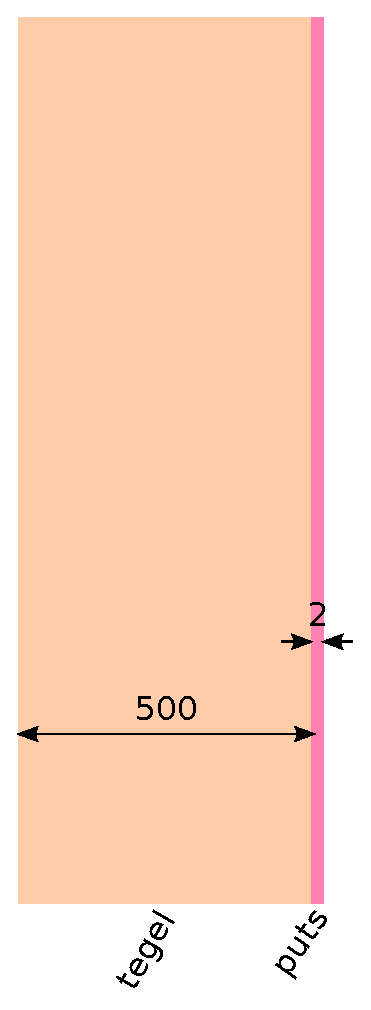
\includegraphics[height=0.3\textheight]{images/sodervagg.eps}
\caption{\label{fig:sodervagg}{Söderväggen, utifrån och in från vänster till höger. Alla mått är i mm.}}
\end{figure}

\begin{figure}[hpbt]
\centering
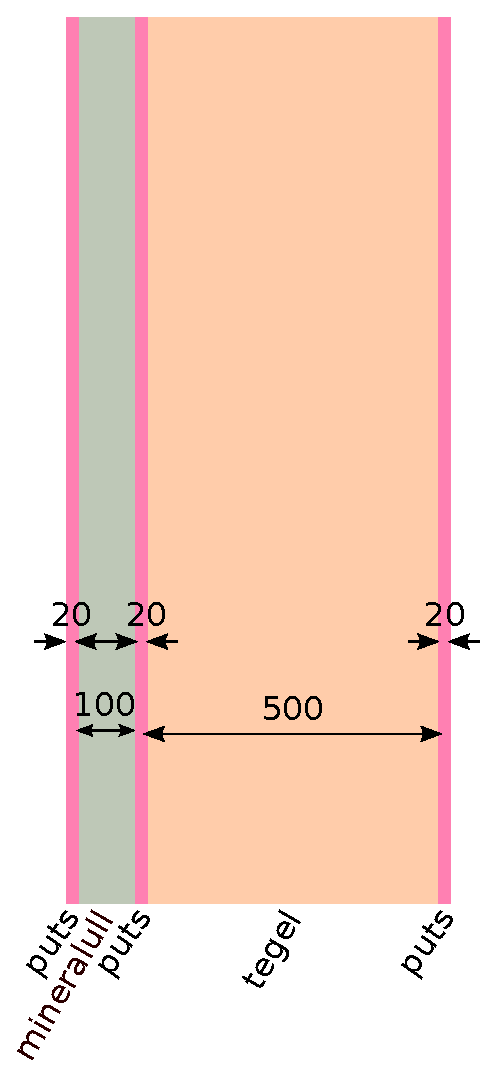
\includegraphics[height=0.3\textheight]{images/norrvagg.eps}
\caption{\label{fig:norrvagg}{Norrväggen, utifrån och in från vänster till höger. Alla mått är i mm.}}
\end{figure}

Fastigheten mellan två andra byggnader i liknande stil. Det öster om är lika högt som fastigheten medan det i väster är något lägre. Fastighetens yttervägg i väster är inte tilläggsisolerad och har samma uppbyggnad som söderväggen, se figur \ref{fig:sodervagg}.

På söderväggen finns ett burspråk som är kopparklätt kopparn sitter direkt på en cementbunden spånskiva och sedan en luftspalt om ca 2,5 cm. Väggen innanför består av 1,6 cm gips, 5 cm minneralull och sedan ytterligare 2,4 cm gips, se figur \ref{fig:bursprak}.\cite{kandidatarbete2010} Enligt Peter Särneö\cite{petersarneo} är det burspråket som läcker mest energi.

\begin{figure}[hpbt]
\centering
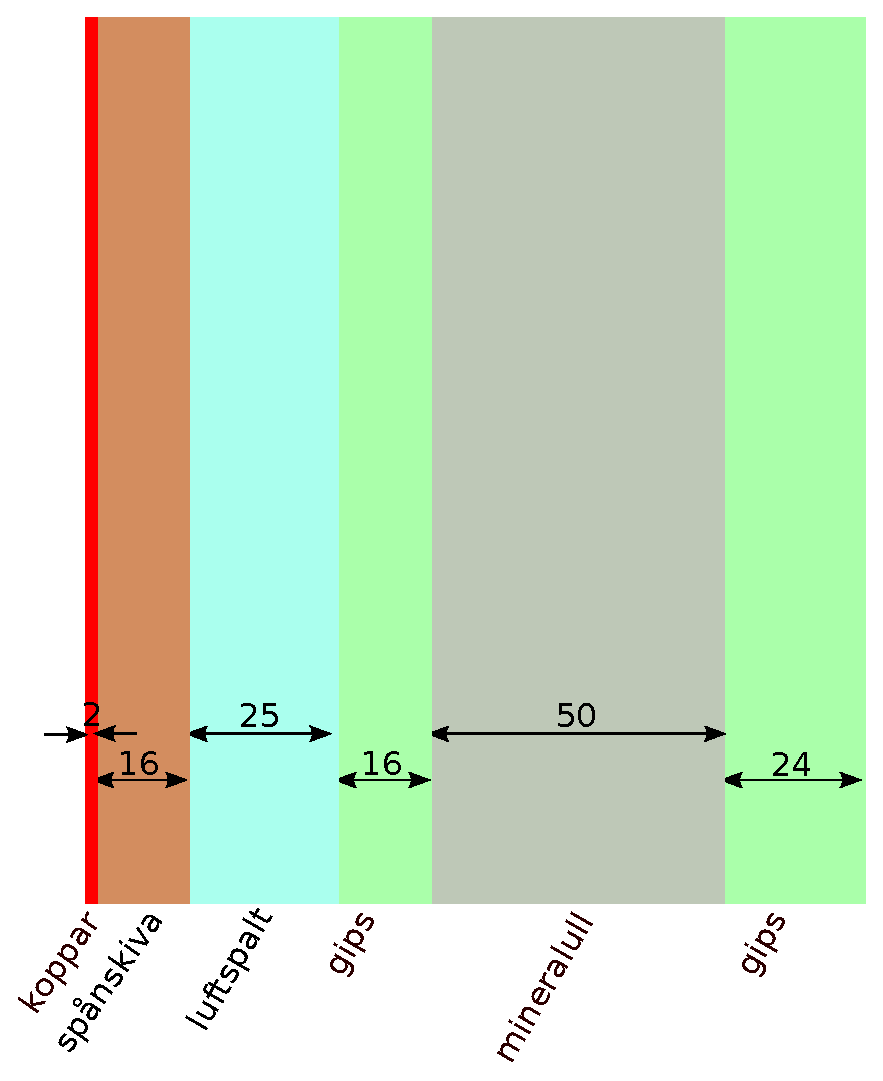
\includegraphics[width=0.3\textheight]{images/bursprak.eps}
\caption{\label{fig:bursprak}{Burspråket på söderväggen, utifrån och in från vänster till höger. Alla mått är i mm.}}
\end{figure}

\subsection{Taket}
Även taket lades om i samband med den stora renoveringen för minskad energiåtgång. Efter det bestod det av taktegel på underlagspapp ytterst, följt av 1,3 cm gips, 21 cm mineralull och innerst ytterligare 2,6 cm gips, se figur \ref{fig:taket}.\cite{kandidatarbete2010}

\begin{figure}[hpbt]
\centering
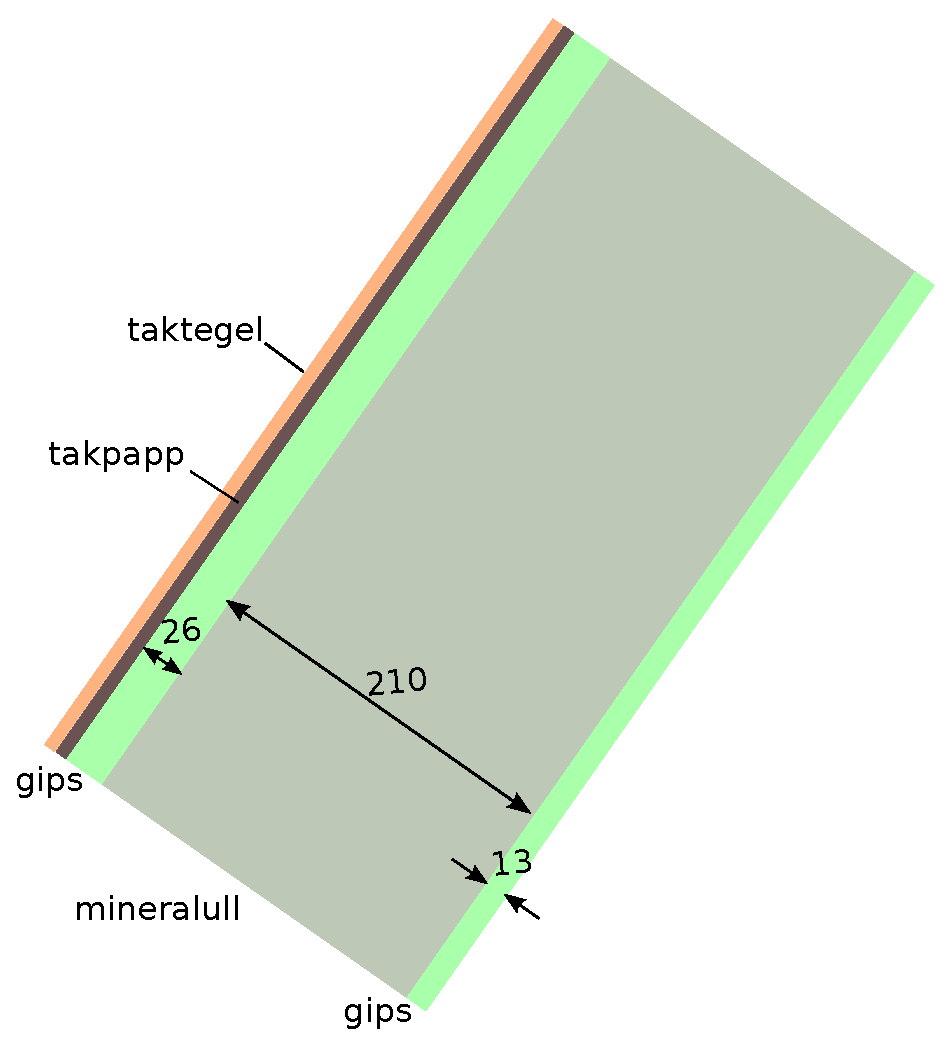
\includegraphics[width=0.3\textheight]{images/taket.eps}
\caption{\label{fig:taket}{Takets uppbyggnad. Alla mått är i mm.}}
\end{figure}

\subsection{Fönstren}

Byggnadens fönster är av treglastyp utan ytbeläggningar. Utrymmet mellan de två innersta glasskivorna är fyllt med argon för att minska värmeledningsförmågan. Totalt får fönstren ett U-värde på ungefär $\unit[1]{W/m^2}$, se avsnitt \ref{sec:heatconduction}. 

\subsection{Grunden}

Huset är byggt på ett berg som sluttar kraftigt. I östra delen av fastigheten ligger huset direkt på berget med endast ett lager av makadam emellan\cite{petersarneo}. I västra halvan har huset en undre källare, det är där apparat- och fläktrummen finns. Där är det betydligt större avstånd ned till berget, uppskattningsvis ett par meter. % Mer exakt? Källa?

\subsection{Uppvärmning och ventilation}
Idag värms huset av bergvärme från tre bergvärmepumpar. För att minska energiåtgången har ett flertal värmeväxlare installerats och värmen från all frånluft återanvänds i möjligaste mån.
% Hur fungerar regleringen? Källa?
Det är viktigt att lägenheterna är kalibrerade så att de får samma temperatur vid samma energiutflöde.


